%\documentclass{article}

\documentclass[12pt,oneside]{article}
\usepackage[a4paper, left=2.5cm, right=2.5cm, top=2.5cm, bottom=1in]{geometry}

\usepackage{amsmath} 
\usepackage{amssymb} 
\usepackage{amstext}
\usepackage{amsthm}

\usepackage{graphicx}
\usepackage{xcolor}

% for bibliography:
\usepackage{comment} 
%\usepackage[ backend=biber, style=chicago ]{biblatex}
\usepackage[
backend=biber,
style=numeric,
]{biblatex}
\DeclareNameAlias{default}{last-first}

\addbibresource{references.bib}
% see:
% https://www.sharelatex.com/learn/Bibliography_management_in_LaTeX#The_bibliography_file

\usepackage[export]{adjustbox}
%\usepackage{tikz}
%\usetikzlibrary{arrows}
%\usetikzlibrary{scopes}
%\usetikzlibrary{babel}

% For cross references 
%\usepackage{hyperref} 
\usepackage[colorlinks = true]{hyperref}
\usepackage[catalan]{varioref}
%\usepackage{cleveref}
%hyperref configuration so that it doesn't contrast so much colorlinks,
\usepackage{xcolor} 
\hypersetup{ 
   linkcolor={black},
   citecolor={black}, 
   %linkcolor={red!50!black},
   %citecolor={blue!50!black}, 
   urlcolor={blue!80!black} }

% Custom Math operators (functions not in italic in math mode):
\DeclareMathOperator{\arcsec}{arcsec} 
\DeclareMathOperator{\arccot}{arccot}
\DeclareMathOperator{\arccsc}{arccsc} 
\DeclareMathOperator{\cis}{cis}

\usepackage[catalan]{babel} %Names in spanish
\usepackage[utf8]{inputenc} %Use unicode
\usepackage[T1]{fontenc}
\usepackage{csquotes} %For bibliography quotations
\DeclareQuoteAlias{spanish}{catalan}

\usepackage{array} 
\usepackage{float}  %Force tables and images position (H and H!)
\usepackage{wrapfig} %Wrap images like in HTML
\usepackage{minted} %For code blocks
\usepackage{color}  %Custom colors for syntax highlight in listings

\usepackage{tabularx,colortbl, booktabs} %Better tables
%\usepackage[alsoload=hep]{siunitx} %Better tables and SI units and uncertainties
\usepackage{longtable}
%\sisetup{separate-uncertainty=true}
%\sisetup{locale = FR} %commas and so on for spanish
%\sisetup{
  %per-mode=fraction,
  %fraction-function=\nicefrac
%}
\usepackage{multirow}
\usepackage{multicol}
\usepackage{makecell}%Slit cell in lines and more formating options inside table

\usepackage{datetime} %To customize date

\newdateformat{monthyeardate}{%
    \monthname[\THEMONTH], \THEYEAR}
%Now \monthyeardate\today gives the date without the day

%\usepackage[framemethod=tikz]{mdframed} 
\usepackage{nicefrac} %nice fractions in one line

%Subfigures
\usepackage{subcaption} 
\usepackage{relsize} %Bigger math with mathlarger{___}

\usepackage[bottom]{footmisc} %footnote at the bottom

%\renewcommand{\figurename}{Fig.} \renewcommand{\tablename}{Tabla}
%tabla-es in babel better

% Add command before appendix session for page numbering: A-1
\newcommand{\appendixpagenumbering}{
    \break
    \pagenumbering{arabic}
    \renewcommand{\thepage}{\thesection-\arabic{page}}
}

\newcommand{\whitepage}{
    \clearpage\thispagestyle{empty}\addtocounter{page}{-1} \newpage \clearpage
}

\setminted{
frame=lines,
framesep=2mm,
baselinestretch=0.2,
fontsize=\footnotesize,
linenos
}

%\addbibresource{Projecte_A.bib}
%\usepackage{graphicx}

\title{Projecte A - Grafs}
\author{
Aleix Boné Ribó\\
Alex Herrero Pons\\
Alex González Godoy\\
Albert Mercadé Plasencia\\
}
\date{Setembre 2019}

\begin{document}

\thispagestyle{empty}
\clearpage
\setcounter{page}{-1}

\begin{titlepage}
{
    \centering
    \null
    \vfill
    {\Large Projecte d'Algorísmia\par}
    \vspace{2em}
    {\Huge \bfseries 
    Transició de fase i components connexes en grafs aleatoris
    \par}
    \vspace{2em}
    {\large \scshape 
    Grau A \qquad Tardor Curs 2019-2020
    \par}
    \vfill
\begin{center}
    
\end{center}
    \vspace{3cm}

    \vfill
    {\raggedleft \large
Aleix Boné Ribó\\
Alex Herrero Pons\\
Alex González Godoy\\
Albert Mercadé Plasencia\\
        \par}
}
\end{titlepage}

\pagebreak
\pagenumbering{Roman} 

\tableofcontents
\pagebreak
\pagenumbering{arabic} 

\section{Introducció}
Per raons d'eficiència hem implementat la classe \texttt{Graph} amb llistes d'adjacència. 

\section{Generació dels Grafs}
\subsection{Random Binomial Graphs}
Per generar un Random Binamial Graph (RBG) ens hem basat en el model d'Erdős-Rényi \cite{Erdos1960OnGraphs,Erdos1959OnI} que per un graf $G=(V,E)$ diu que

\begin{equation}
    \forall u,v \in V,\quad (u,v) \in E \text{ amb probabilitat } p
\end{equation}

Hem implementat l'algoritme prèviament descrit sota la funció \texttt{BRG}\footnote{Implementada a src/graph\_generator.cpp}. Per cada vèrtex veiem totes les possible arestes i seguint una distribució de Bernoulli amb probabilitat $p$ decidim quines afegim i quines no.

\subsection{Random Geometric Graphs}
Un Random Geometric Graphs (RGG)\cite{Diaz2007On} per tot vèrtex $v \in V$ li assignem unes coordenades ($x_v, y_v$) aleatòries entre 0 i 1. Cada vèrtex 

\begin{align}
    \forall u,v \in V,\quad (u,v) \in E \Longleftrightarrow \text{dist}(u,v) &\leq r \\
    \text{dist}(u,v) &= \sqrt{\left(x_v - x_u\right)^2 + \left(y_v - y_u\right)^2}
\end{align}

\section{Càlcul de Components Connexos}

\section{Càlcul Adaptatiu}

\section{Anàlisis de Resultats}

\begin{figure}[H]
    \centering
    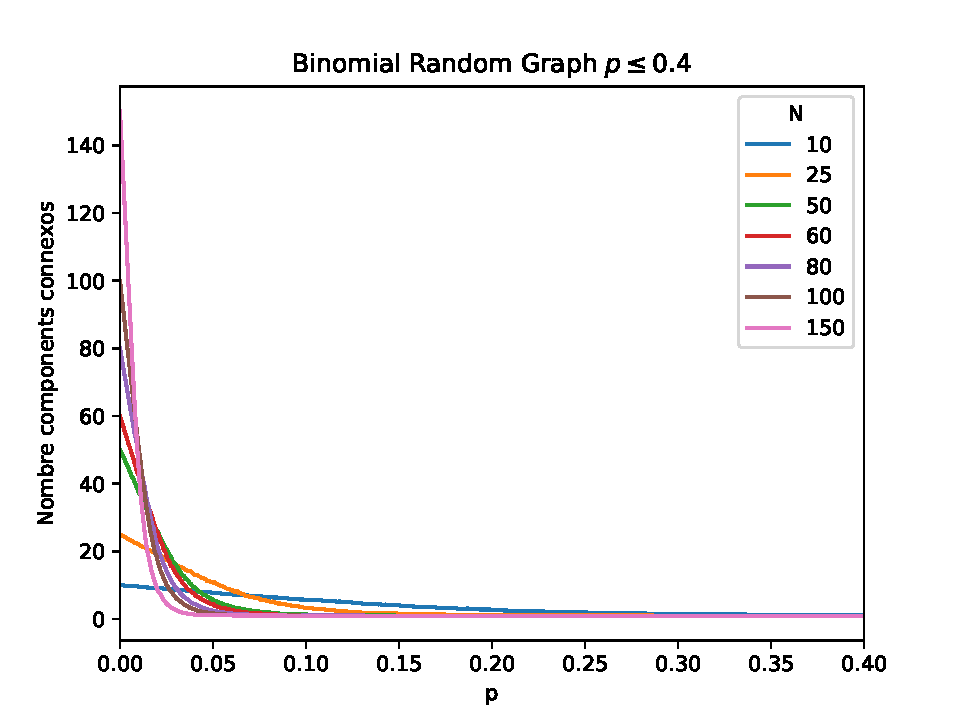
\includegraphics[width=10cm]{plots/bin_mult_2_04.pdf}
    \caption{Connectivitat de BRG per diferents valors de n}
    \label{fig:connect_04}
\end{figure}

\begin{listing}
\inputminted{cpp}{src/graph.h}
\caption{test}
\label{lst:test}
\end{listing}

\pagebreak

\printbibliography

\end{document}
